\documentclass[12pt, a4paper]{article}

\usepackage{fancyhdr}
\usepackage[left=4cm, right=4cm, top=4cm, bottom=4cm]{geometry}
\usepackage[utf8]{inputenc}
\usepackage{amsmath, amssymb, amsthm, amsfonts}
\usepackage{graphicx}
\usepackage{float}
\usepackage{hyperref}
\usepackage{listings}
\usepackage{color}
\usepackage{subcaption}
\usepackage{enumitem}
\usepackage{mathtools}
\usepackage{bbm}
\usepackage{cite}
\newcommand{\coursename}{EE 541 Computational Introduction to Deep Learning}
\newcommand{\doctitle}{American Sign Language (ASL) Alphabet Classification}
\newcommand{\name}{Abid Hassan, Benjamin Fein-Ashley}
\newcommand{\todaydate}{\today}
\DeclareMathOperator*{\argmin}{arg\,min}
\DeclareMathOperator*{\argmax}{arg\,max}

% \pagestyle{fancy}
% \lhead{\textbf{\doctitle}}
% \chead{\name}
% \rhead{\todaydate}

\begin{document}


\begin{center}
\small
\textbf{\coursename} \\
\Large
\bfseries
\doctitle \\
\vspace{0.8cm}
\small
{\normalfont\small \name}
\end{center}

\thispagestyle{plain}

\noindent

\newpage

\begin{section}{Introduction}
    In this work, we utilize several deep learning algorithms to classify American Sign Language (ASL) alphabet letters from images, as well as real-time classification using live video. The dataset used for this project is the ASL Alphabet dataset \cite{kaggle2022aslalphabet}, which contains images of hand signs representing each letter of the ASL alphabet. The goal is to build a model that can accurately classify these hand signs into their corresponding letters.
    We examine ResNet18 and DenseNet121 architectures, and compare their performance in terms of accuracy on a test dataset. The provided training dataset is split into 90 percent training and 10 percent test data, as the provided test set contains only one image per class. The whole data set contains 87,000 images which are 200x200 pixels, so 78,300 images are used in training and 8,700 for testing (300 per class). There are 29 classes, of which 26 are for the letters A-Z and 3 classes for space, delete, and nothing, which are intended to improve performance in real time classification.
    
    \subsection{Literature Review}
    A variety of machine learning and deep learning methods have been applied to sign language recognition with varying success.
    Principal Component Analysis (PCA) combined with SVM classification achieved around 94\% accuracy, demonstrating a baseline for evaluating more complex deep learning architectures \cite{mdpi2023resnet}.
    
    A study utilizing multiple deep learning models, including ResNet-50 and EfficientNet, showed significant success using transfer learning techniques, achieving accuracies up to 99.98\% with ResNet-50 \cite{mdpi2023resnet}.
    
    MobileNetV2 was employed as a lightweight architecture, achieving 98.77\% accuracy, suitable for real-time classification on resource-constrained devices \cite{techscience2022mobilenet}.
    
    A novel hardware-based approach used neuromorphic sensors coupled with an artificial neural network implemented on an FPGA, achieving 79.58\% accuracy \cite{mdpi2017neuromorphic}. Although the accuracy of this method is lower than others, it represents a more practical system for real time application.
    
    \begin{table}[H]
    \centering
    \caption{Accuracy Results from the Literature Review}
    \label{tab:litreview}
    \begin{tabular}{|l|c|}
    \hline
    Model & Accuracy (\%) \\
    \hline
    ResNet-50 (Transfer Learning) \cite{mdpi2023resnet} & 99.98 \\
    MobileNetV2 \cite{techscience2022mobilenet} & 98.77 \\
    Neuromorphic Approach \cite{mdpi2017neuromorphic} & 79.58 \\
    PCA + SVM \cite{mdpi2023resnet} & 94.00 \\
    \hline
    \end{tabular}
    \end{table}
    Although computationally expensive, ResNet models are able to achieve near perfect classification on the ASL test dataset. Several lightweight and embedded architectures also achieve high accuracy. Non deep-learning methods such as PCA + SVM have lower accuracy.

\end{section}

\begin{section}{Methods}
    \subsection{Data Preprocessing}
    First, the data is split into 90 percent training and 10 percent for testing. The data is then preprocessed by resizing the images to a uniform size of 200x200 pixels and normalizing the pixel values to be between 0 and 1. Data augmentation techniques such as rotation, flipping, and zooming are applied to increase the diversity of the training data and improve the model's generalization ability.
    \begin{table}[H]
        \centering
        \caption{Overview of Data Split and Image Specifications}
        \label{tab:datasplit}
        \begin{tabular}{|l|cl|}
        \hline
        \textbf{Category} & \textbf{Number of Images} & \textbf{Percentage} \\
        \hline
        Overall Dataset & 87,000 & 100\% \\
        Training Set & 78,300 & 90\% \\
        \quad Training (90\%) & 62,640 & 72\% \\ 
        \quad Validation (10\%) & 15,660 & 18\% \\ 
        Test Set & 8,700 & 10\% \\
        \hline
        \end{tabular}
        \end{table}
    \subsection{Model Architecture}
    We implement two deep learning architectures,  ResNet18, and DenseNet121. These architectures are chosen for their proven performance in image classification tasks. The models are trained using the Adam optimizer with a learning rate of 0.01 and a batch size of 64. The loss function used is categorical cross-entropy.
    ResNet (Residual Network) employs skip (or residual) connections that allow the network to bypass one or more layers. This design aids in mitigating the vanishing gradient problem, thus facilitating the training of very deep networks. In contrast, DenseNet (Dense Convolutional Network) creates direct connections between all layers within a dense block, where each layer receives the concatenated output of all preceding layers. This dense connectivity enhances feature reuse and typically results in improved parameter efficiency.
    
    For comparison to non-deep learning methods, we also implement an SVM classifier with PCA dimensionality reduction. The PCA is set up to keep 95\% of the variance in the data, and the SVM is trained using a radial basis function (RBF) kernel.
    \subsection{Training and Evaluation}
    The models are trained on the training dataset for 20 epochs. The provided training data is randomly split in an 80 to 20 ratio of training to validation data. The model at the epoch with best validation accuracy is saved as the final model to be evaluated. The performance of each model is evaluated on a separate test dataset, and metrics such as accuracy, precision, recall are calculated.
    The data is split into 80 percent training and 20 percent validation. The test set is provided separately from the training data.
\end{section}

\begin{section}{Results}
    The results of the experiments are summarized in Table \ref{tab:results}. 
    \begin{table}[H]
        \centering
        \caption{Model Performance on Test Dataset}
        \label{tab:results}
        \begin{tabular}{|c|c|c|c|c|}
            \hline
            Model & Test Accuracy & Precision & Recall \\
            \hline
            SVM + PCA & 89.3\%& 0.88 & 0.89 \\
            ResNet18 &100\% & 1.0 & 1.0 \\
            % ResNet34 & --\% & -- & --  \\
            % ResNet50 & --\% & -- & --  \\
            DenseNet121 & 99.98\% & 1.0 & 1.0  \\
            \hline
        \end{tabular}
    \end{table}
    The ResNet18 model achieved perfect accuracy on the test set, while DenseNet121 achieved almost perfect accuracy, misclassifying two images in the test set. SVM + PCA performed significantly worse. The SVM architecture is less capable of capturing local features in the images, limiting its performance.
    \begin{figure}[H]
        \centering
        \begin{subfigure}[b]{0.45\textwidth}
            \centering
            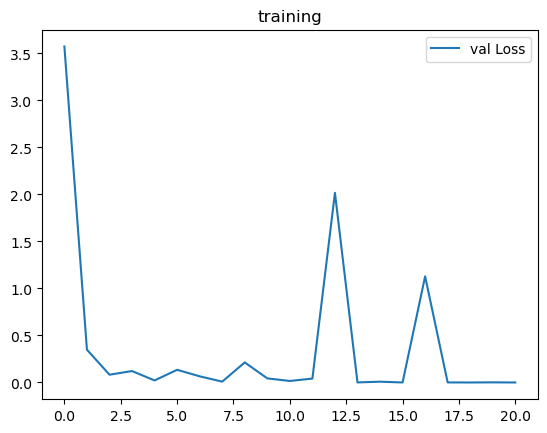
\includegraphics[width=\textwidth]{../plots/ResNet18_training.png}
            \caption{ResNet18 Training Loss}
            \label{fig:resnet18_training}
        \end{subfigure}
        \hfill
        \begin{subfigure}[b]{0.45\textwidth}
            \centering
            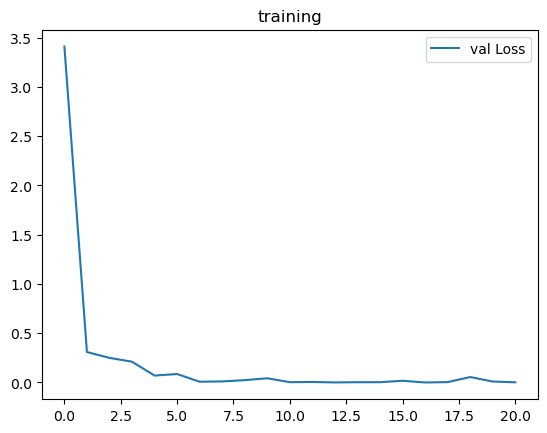
\includegraphics[width=\textwidth]{../plots/DenseNet121_training.png}
            \caption{DenseNet121 Training Loss}
            \label{fig:densenet121_training}
        \end{subfigure}
        \caption{Training Loss Comparison for ResNet18 and DenseNet121}
        \label{fig:training_loss}
    \end{figure}
    \begin{figure}[H]
        \centering
        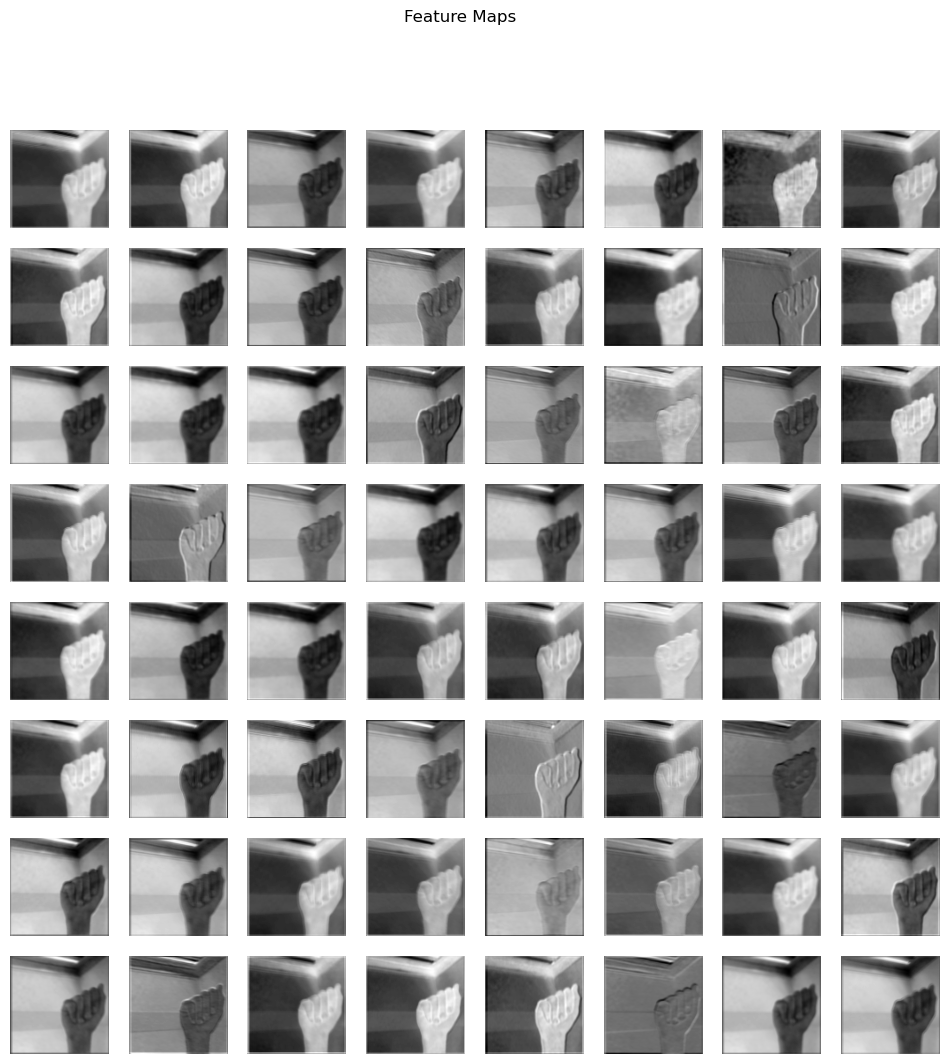
\includegraphics[width=0.5\textwidth]{../plots/ResNet18_Visualize.png}
        \caption{Feature Maps from the ResNet18 model}
        \label{fig:resnet18_visualize}
    \end{figure}
    \begin{figure}[H]
        \centering
        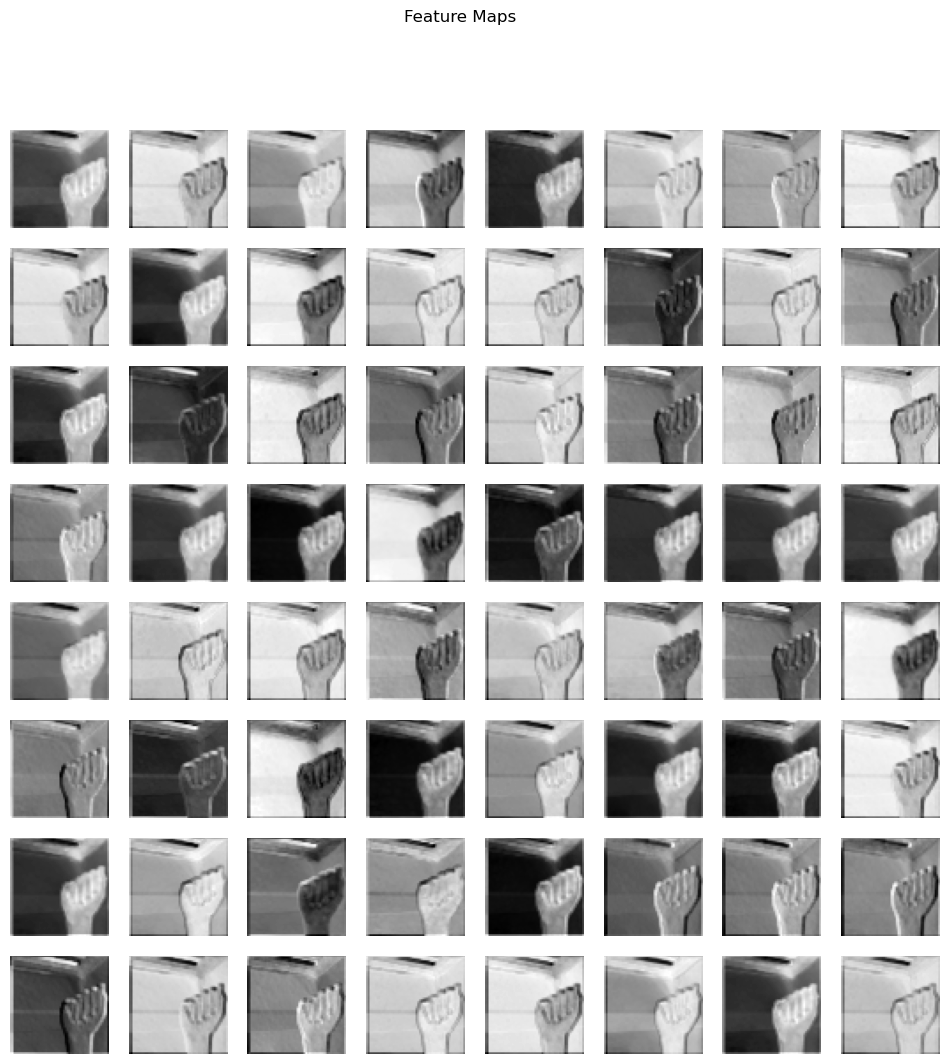
\includegraphics[width=0.5\textwidth]{../plots/DenseNet121_Visualize.png}
        \caption{Feature Maps from the DenseNet121 model}
        \label{fig:densenet121_visualize}
    \end{figure}
    The models were also tested on live video input, achieving real-time classification. The input utilizes a webcam and a defined bounding box to classify signs made by the user.
    \begin{figure}[H]
        \centering
        \begin{subfigure}[b]{0.45\textwidth}
            \centering
            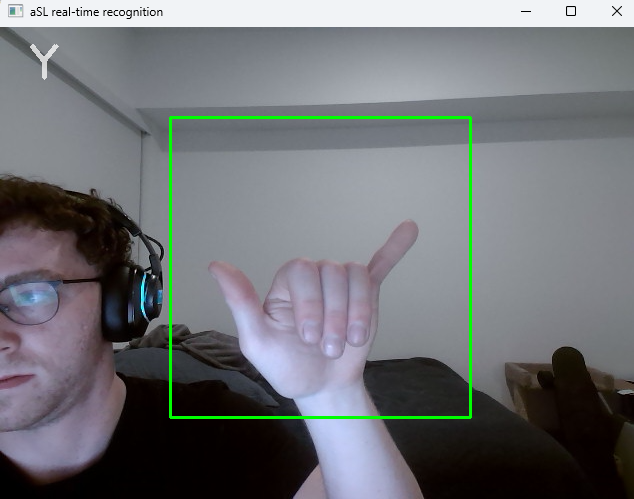
\includegraphics[width=\textwidth]{../plots/real_time_sample.png}
            \caption{Signing "Y"}
            \label{fig:signY}
        \end{subfigure}
        \hfill
        \begin{subfigure}[b]{0.45\textwidth}
            \centering
            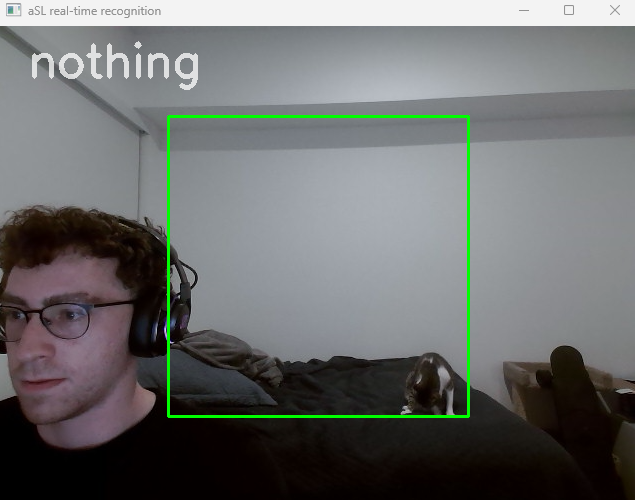
\includegraphics[width=\textwidth]{../plots/real_time_sample2.png}
            \caption{Nothing}
            \label{fig:nothing}
        \end{subfigure}
        \caption{Example live classification of video input}
        \label{fig:live_video_samples}
    \end{figure}
\end{section}

\begin{section}{Conclusion}
    \subsection{Extensions/Challenges}
    There were few challenges in terms of the performance of deep learning models on this dataset. Our ResNet18 transfer learning model achieved perfect accuracy on the test set, and our DenseNet121 model was also very close to perfect. This accuracy is very similar to literature accuracies for these models. The challenge for this dataset comes from creating lightweight models that can be used in real time or embedded systems. We used our model for live classification, which works fairly well but is far from perfect. More work could be done on processing the real time image so it is ready for classification, such as learning to place the bounding box in the correct position. Currently the software requires careful hand positioning to generate accurate classification, which is not ideal for a final product. Labels are generated very quickly and there is not a noticeable delay for live classification.
    \subsection{Final Remarks}
    The project successfully demonstrates the application of deep learning models for ASL classification. The ResNet18 and DenseNet121 architectures achieved high accuracy, making them suitable for real-time applications. Future work could focus on improving the robustness of the models in real-world scenarios, such as varying lighting conditions and hand positioning.
\end{section}
\bibliographystyle{IEEEtran}
\bibliography{references}
\end{document}




